\subsection{阿廷环与诺特环}

定义 2. --- 称环 A 为左阿廷（相应地，左诺特）环，如果左 A-模 \(A_{s}\) 是阿廷（相应地，诺特）的。同样，称环 A 为右阿廷（相应地，右诺特）环，如果右 A-模 \(A_{d}\) 是阿廷（相应地，诺特）的。

环 A 是右阿廷（相应地，右诺特）的，当且仅当它的反环 \(A^{o}\) 是左阿廷（相应地，左诺特）的。对交换环 A，左阿廷与右阿廷这两条性质重合；当它们成立时，我们说环 A 是阿廷环；对``诺特''我们采用类似的约定。存在左阿廷而非右阿廷的非交换环，也存在左诺特而非右诺特的非交换环（VIII, p.~14, 习题 3）。

设 \(A\) 为环。按定义，下列性质等价：

\begin{enumerate}
\def\labelenumi{(\roman{enumi})}
\item
  环 A 是左阿廷的。
\item
  A 的左理想的任一非空集合按包含关系排序都有一个极小元。
\item
  A 的左理想的任一递减序列都是平稳的。
\end{enumerate}

由于 VIII, p.~3 的命题 2，下列性质等价：

\begin{enumerate}
\def\labelenumi{(\roman{enumi})}
\item
  环 A 是左诺特的。
\item
  A 的左理想的任一非空集合按包含关系排序都有一个极大元。
\item
  A 的左理想的任一递增序列都是平稳的。
\item
  A 的每个左理想都由 A 的一个有限子集生成。
\end{enumerate}

例. --- 1) 体是既左且右阿廷、又诺特的环。

\begin{enumerate}
\def\labelenumi{\arabic{enumi})}
\setcounter{enumi}{1}
\item
  设 A 为环，D 为 A 的子环。假设 D 是体且 A 是 D 上的有限维左向量空间。则环 A 是左阿廷且左诺特的，因为 A 的每个左理想都是 A 的 D-向量子空间。特别地，交换域上的有限维代数是既左且右阿廷、又诺特的环。
\item
  主理想整环（VII, §1, No.~1, p.~1, 定义 1）是诺特的。不是体的整环 A 不是阿廷环：对 A 的每个非零且不可逆的元素 \(a\) ，理想序列 \(a^n\mathbf{A}\) （对 \(n \in \mathbf{N}\) ）严格递减。特别地，整数环 \(\mathbf{Z}\) 是诺特的但不是阿廷的。
\item
  设 M 为 A-模，它是非零子模的无穷族 \((\mathrm{M}_{i})_{i\in\mathrm{I}}\) 的直和。设 E 为 M 的自同态环。对每个 \(i\in I\) ，设 \(a_{i}\) （相应地，\(b_{i}\) ）为 E 中核包含 \(\sum_{j\neq i}M_{j}\) （相应地，像含于 \(M_{i}\) ）的元素组成的集合。则 \((a_{i})\) 是 E 的非零左理想的无穷族，其和是直和；\((b_{i})\) 是 E 的非零右理想的无穷族，其和是直和。因此，环 E 既非左亦非右阿廷（相应地，诺特）的（VIII, p.~2, 例 2）。特别地，无穷维向量空间的自同态环既非左亦非右阿廷（相应地，诺特）。
\end{enumerate}

定理 1. --- 设 A 为左阿廷环。则 A-模 \(A_{s}\) 具有有限长度。

证明中我们将使用下面的引理。

引理 3. --- 设 A 为环，n 为自然数。阿廷 A-模 M 若是长度 \(\leqslant n\) 的子模的一个族的和，则具有有限长度。

对 n 用归纳法。~首先设 n = 1。若 M 不是有限长度的，则可以构造 M 的长度为 1 的子模的序列 \((\mathrm{M}_{m})_{m \in \mathbf{N}}\) ，使得 \(M_{m} \not\subset (\sum_{i < m} M_{i})\) 对每个 \(m \in N\) 成立。于是对每个 m 有 \(M_{m} \cap \sum_{i < m} M_{i} = 0\) ，从而族 \((\mathrm{M}_{m})_{m \in \mathbf{N}}\) 的和是直和。然而这与 A-模 M 是阿廷的这一事实矛盾（VIII, p.~2, 例 2）。

现设 \(n \geqslant 2\) 。设 \((\mathrm{M}_{i})_{i \in \mathrm{I}}\) 为 M 的长度 \(\leqslant n\) 的子模的族，其和为 M。对每个 \(i \in I\) ，选取子模 \(M_{i}^{\prime}\) （它含于 \(M_{i}\) ，长度 \(\leqslant n - 1\) ），使 \(M_{i}/M_{i}^{\prime}\) 的长度 \(\leqslant 1\) 。置 \(M^{\prime} = \sum M_{i}^{\prime}\) ，并把 \(M_{i}\) 在 \(M^{\prime\prime} = M/M^{\prime}\) 中的像记作 \(M_{i}^{\prime\prime}\) 。诸模 \(M_{i}^{\prime\prime}\) 的长度 \(\leqslant 1\) ，且其和为 \(M^{\prime\prime}\) 。诸模 \(M^{\prime}\) 与 \(M^{\prime\prime}\) 都是阿廷的（VIII, p.~3, 命题 3）；由归纳假设，它们都是有限长度的。于是 M 具有有限长度（II, §1, No.~10, p.~212, 命题 16）。

现在来证明定理 1。用 S 表示使模 \(A_{s}/a\) 具有有限长度的 A 的左理想 a 组成的集合。设 \((\mathfrak{a}_{i})_{i\in I}\) 为 S 的元素的有限族。由 VIII, p.~2 的命题 1，A-模 \(A_{s}/a_{i}\) 对每个 \(i\in I\) 都是阿廷且诺特的。因此，\(A_{s}/\bigcap_{i\in I}a_{i}\) 是阿廷且诺特的（VIII, p.~4, 命题 3 的推论），从而具有有限长度（VIII, p.~2, 命题 1）。这就证明 S 关于包含关系是左向定向集。由于环 A 是左阿廷的，集合 S 有一个最小元 b。我们用 n 表示 A-模 \(A_{s}/b\) 的长度。

设 \(x\) 为 \(A_s\) 的元素，\(\mathfrak{a}\) 为其零化子（II, §1, No.~12, p.~219）。A-模 \(Ax\) 同构于 \(A_s / \mathfrak{a}\) 。若 \(Ax\) 具有有限长度，则 \(\mathfrak{a}\) 属于 \(\mathscr{S}\) ，于是 \(\mathfrak{a}\) 包含 \(\mathfrak{b}\) ，而 \(Ax\) 的长度 \(\leqslant n\) 。这样，\(A\) 的每个具有有限长度的单生成左理想的长度都 \(\leqslant n\) 。设 \(\mathfrak{c}\) 为这些理想的和；由引理 3，它是 \(A\) 的一个有限长度左理想。\(A\) 的每个有限长度左理想都是有限长度单生成左理想的和，因而含于 \(\mathfrak{c}\) 。于是，\(\mathfrak{c}\) 是 \(A\) 的最大的有限长度左理想。

若 c 异于 A，则 A 的包含 c 且异于 c 的左理想组成的集合将有一个极小元 \(c'\) 。于是 A-模 \(c'/c\) 的长度将为 1，而 \(c'\) 将具有有限长度，这与 c 的最大性矛盾。因此有 c = A；A-模 \(A_{s}\) 具有有限长度。

推论. --- 每个左阿廷环都是左诺特的。

设 \(A\) 为左阿廷环。由定理 1，\(A\) -模 \(A_s\) 具有有限长度。然后应用 VIII, p.~2 的命题 1。

设 A 为左（相应地，右）阿廷环；A-模 \(A_{s}\) （相应地，\(A_{d}\) ）的长度（I, §4, No.~7, p.~44）称为环 A 的左（相应地，右）长度。当 A 是交换阿廷环时，这两个长度重合，简称为 A 的长度。当 A 既左且右阿廷但不交换时，A 的左长度与右长度不一定相等（VIII, p.~14, 习题 3）。

例 5. --- 体的左长度与右长度都等于 1。

命题 4. --- a) 设 A 为左诺特环，M 为有限生成左 A-模。则模 M 是诺特的，且 M 的每个子模都是有限生成的。

\begin{enumerate}
\def\labelenumi{\alph{enumi})}
\setcounter{enumi}{1}
\tightlist
\item
  设 A 为左阿廷环，M 为左 A-模。下列性质等价：模 M 是有限生成的；模 M 是阿廷的；模 M 具有有限长度；模 M 是诺特的。
\end{enumerate}

我们来证明 a)。M 的每个单生成子模都同构于 \(A_{s}\) 的一个商，故由 VIII, p.~3 的命题 3 是诺特的。模 M 是这类子模的有限和；因此由命题 3 的推论（VIII, p.~4）是诺特的。于是 M 的每个子模都是有限生成的（VIII, p.~3, 命题 2）。

现设环 A 是左阿廷的。与上一节一样可以看出，若 A-模 M 是有限生成的，则它是阿廷的。若它是阿廷的，则它具有有限长度：事实上，它的单生成子模同构于 \(A_{s}\) 的商，因此其长度有限且小于 \(A_{s}\) 的长度，而结论由引理 3 得出。每个有限长度的模都是诺特的，而每个诺特模都是有限生成的。这就证明了 b)。

命题 5. --- a) 设 A 为左阿廷（相应地，左诺特）环，\(\varphi : \mathrm{A} \to \mathrm{B}\) 为使 B 成为有限生成左 A-模的环同态。则环 B 是左阿廷（相应地，左诺特）的。

\begin{enumerate}
\def\labelenumi{\alph{enumi})}
\setcounter{enumi}{1}
\item
  设 A 为左阿廷（相应地，左诺特）环，\(\mathfrak{a}\) 为 A 的双边理想；则环 A/ \(\mathfrak{a}\) 是左阿廷（相应地，左诺特）的。
\item
  设 \((\mathrm{A}_i)_{i\in \mathrm{I}}\) 为左阿廷（相应地，左诺特）环的族。则环 \(\prod_{i\in \mathrm{I}}\mathrm{A}_i\) 是左阿廷（相应地，左诺特）的。
\end{enumerate}

我们将处理阿廷环的情形；诺特环的情形是类似的。

我们来证明 a)。由命题 4，环 \(\mathrm{B}_s\) 是阿廷左 A-模，从而更是阿廷左 B-模。

断言 b) 由断言 a) 应用于从 A 到 A/a 的典范同态而得出。

我们来证明 c)。置 \(A = \prod_{i \in I} A_i\) 。由假设，\((\mathrm{A}_i)_s\) 是阿廷左 \(A_i\) -模，从而更是阿廷左 A-模。由 VIII, p.~4 的例 5，A-模 \(A_s\) 是阿廷的。

推论. --- 阿廷交换环的素理想就是它的极大理想。

在任何交换环中，极大理想都是素的。设 A 为阿廷交换环，p 为 A 的素理想。环 A/p 是整环且是阿廷的（命题 5），故是体（VIII, p.~5, 例 3）。因此，理想 p 是极大的。

\pandocbounded{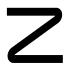
\includegraphics[keepaspectratio]{images/part001_e30b1f1b.jpg}}

多项式环 \(\mathbf{Q}[(\mathrm{X}_{n})_{n\in\mathbf{N}}]\) 是整环；它不是诺特的（也不是阿廷的）（VIII, p.~15, 习题 9）。它是它的分式域的子环，而该分式域是阿廷（且诺特）环。

